% kuleuventheme2poster by Janez Kren, June 2018, janez.kren@kuleuven.be

\documentclass{beamer}
\usepackage[orientation=portrait,size=a3,scale=1.8,debug]{beamerposter}
% BEAMERPOSTER OPTIONS:
%	orientation= portrait / landscape
%	size= a0 / a2 / a3 / a4
%	scale = change the size of text (e.g. 1.4 increases all fonts by factor of 1.4)


\usetheme[sedes]{kuleuven2poster}
% THEME OPTIONS 
%	for logo:   kul (default) / kulak / lrd
%	background colour:   blue (default) / white
%	background sedes logo:   no (default) / sedes
%  e.g. [lrd,white,sedes]


% USE YOUR BACKGROUND IMAGE (optinal):
%\titlegraphic{ \includegraphics[height=0.9\paperheight]{mybackground.jpg} } %or, depending on the size: [width=\paperwidth]
%\def\backgdopacity{0.25}  % background image opacity fraction (0=transparent, 1=full colour)



\usepackage[utf8]{inputenc}
\usepackage{ragged2e}


% INFO 
\title{CoaCo}
\author{\large Olivier Van den Eede, Dylan Van Assche, C\'edric Gullentops, Anton Peeters, Simon Vandevelde}
\institute{\large Faculteit Industriële ingenieurswetenschappen / Elektronica - ICT}
%\date{\large \today}
 

\begin{document}
\csname beamer@calculateheadfoot\endcsname %recalculate head and foot dimension

\begin{frame}[t]

%%
%%  TITLE (optional)
%%
\vspace{2.5\baseh} % extra vertical space

%\begin{tikzpicture}
%\node [text width=\textwidth, text ragged, inner sep=0pt, outer sep=0, kul-blue, font=\bfseries\fontsize{0.6\baseh pt}{2}\selectfont] 	
%{ \inserttitle } ;
%% This will create title larger than \Huge. Replace with the line below, to make it smaller or fine-tune.
%\end{tikzpicture}

%\textcolor{kul-blue}{\bfseries \Huge \inserttitle}



%%
%% BODY
%%
\vspace{.4\baseh}
\begin{columns}[t]
%COLUMN 1
	\begin{column}{\textwidth}

        % Start titel
	\begin{beamercolorbox}{whitebox}
	\justifying
	{\bfseries Het idee}
	
	Onze robot zal blikjes die op kamertemperatuur zijn zoeken, oppakken, en in de pullenbak plaatsen.

	Hiervoor gaat het gebruik maken van deze stappen:
	\begin{figure}
	  \centering
	  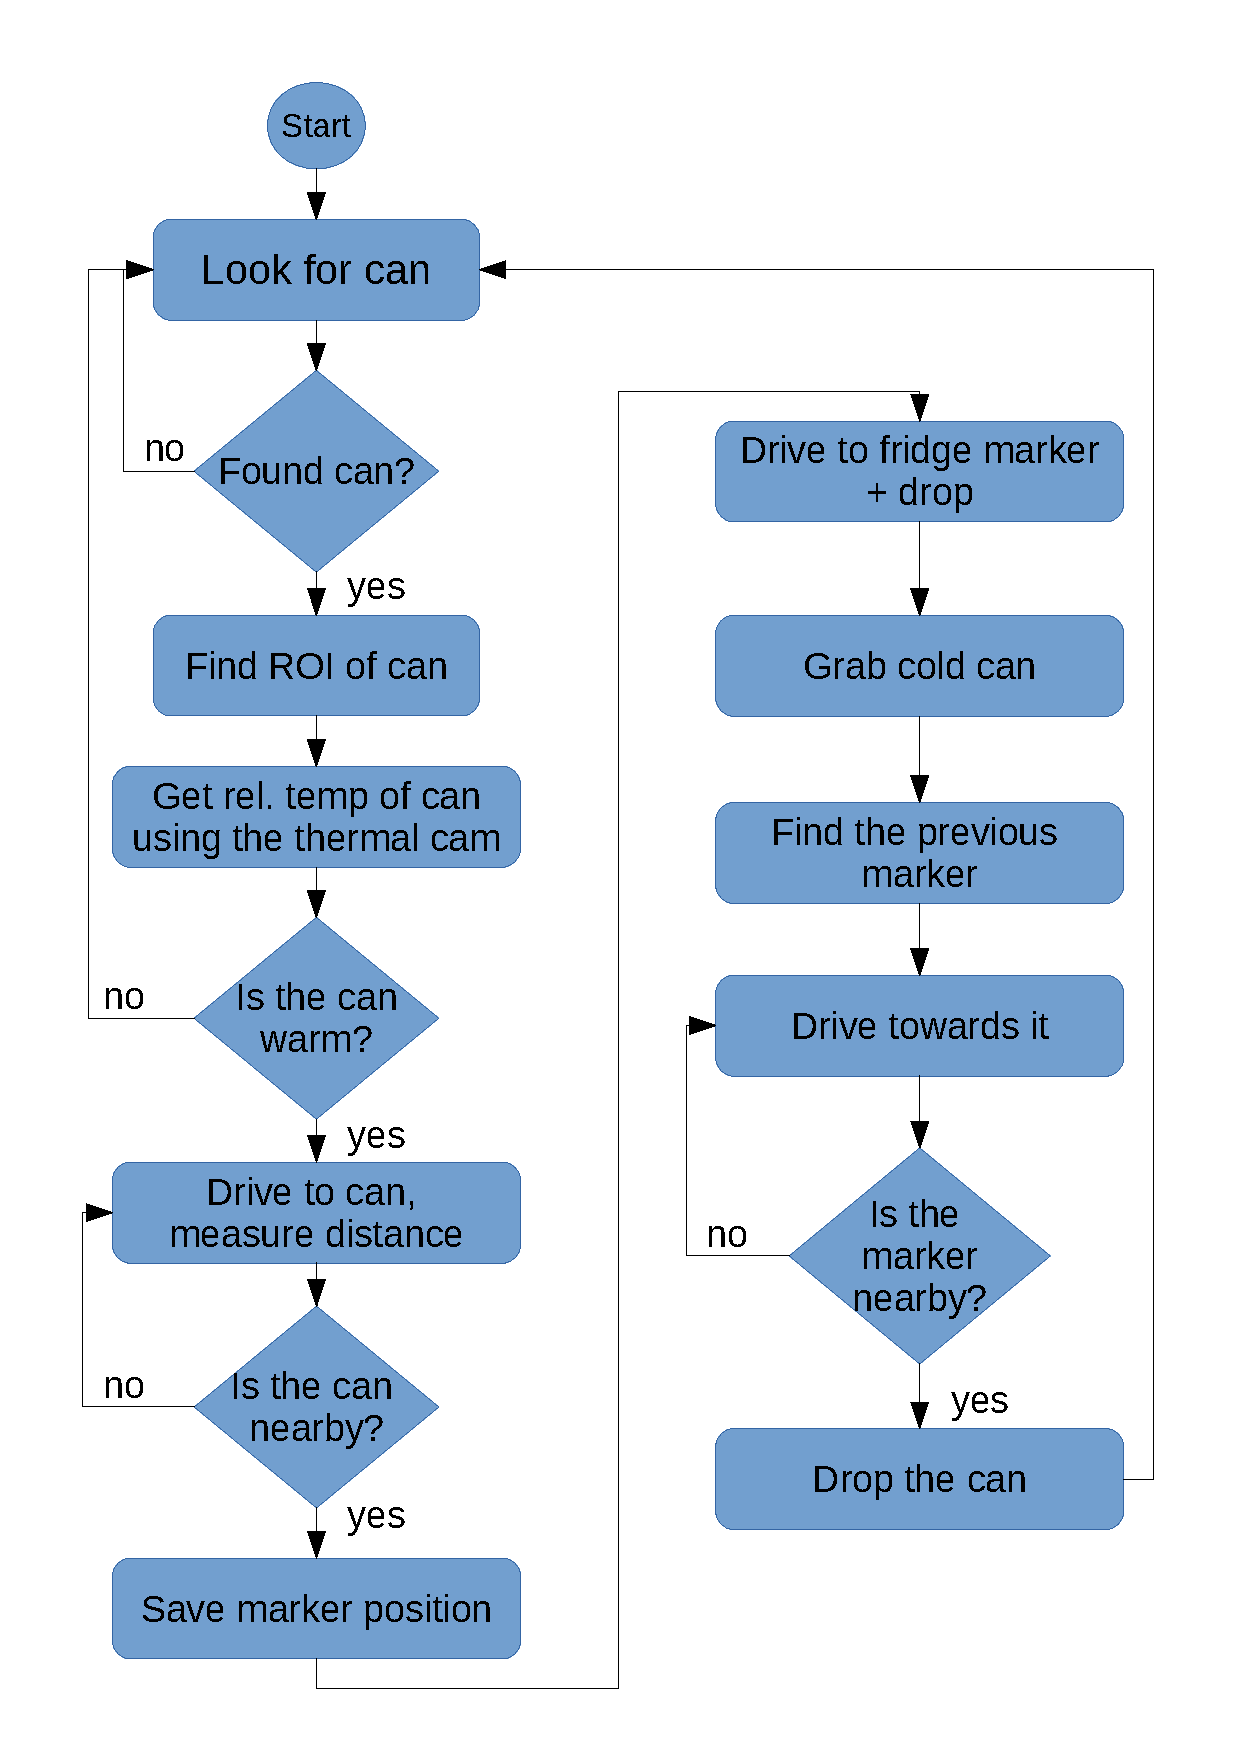
\includegraphics[width=0.9\textwidth]{../../Docs/general_flow.pdf}
	  \caption{Flowchart van het proces}

	\end{figure}

	\vspace{0.5em}
	
        Om dit in de praktijk toe te passen, heeft de robot nood aan bepaalde accesoires.
        Deze zijn:
        \begin{enumerate}
            \item 
        \end{enumerate}
	%Dit wordt gerealiseerd aan de hand van volgende nodes:
	%\begin{figure}
	% \begin{beamercolorbox}{whitebox}
	%  \centering
	%  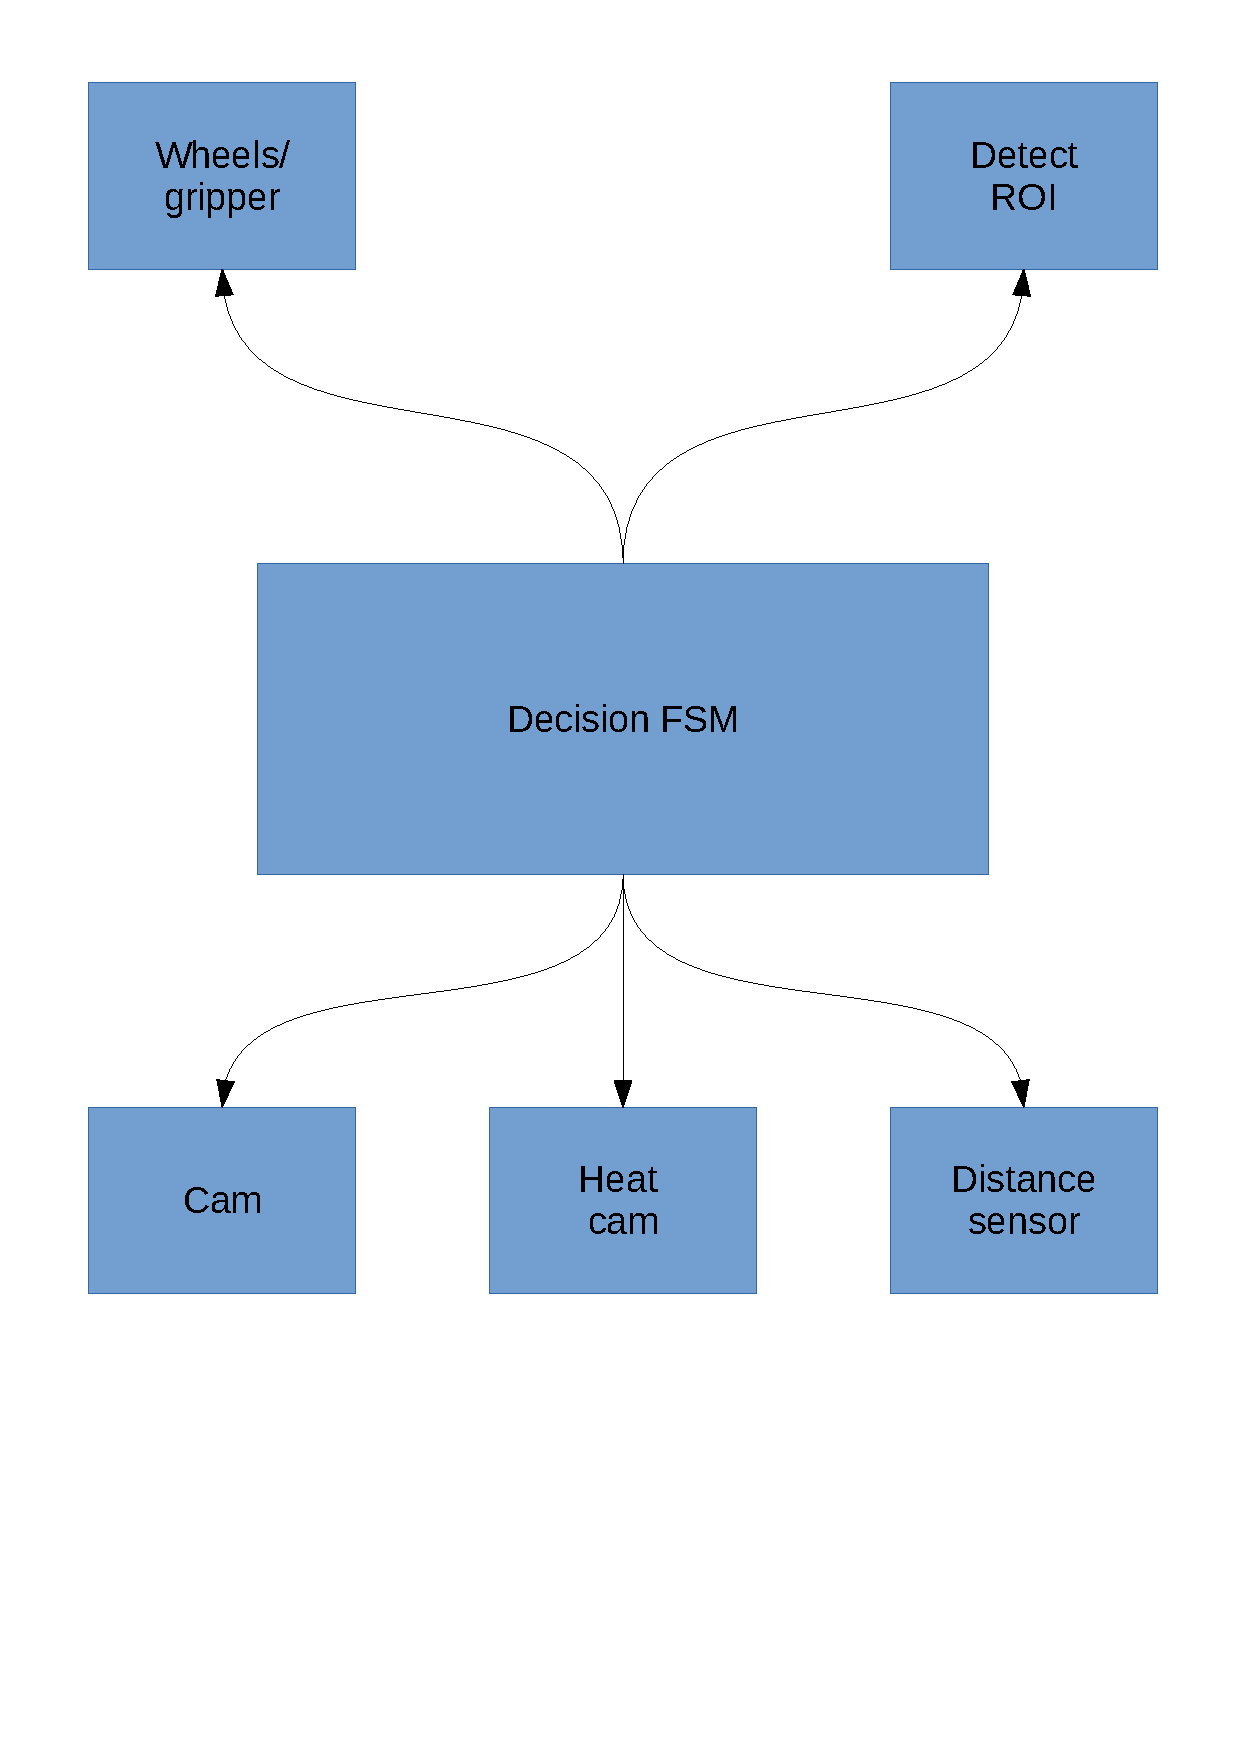
\includegraphics[width=0.7\textwidth]{../../Docs/node_diagram.pdf}
	%  \caption{Nodediagram van nodige nodes}
	% \end{beamercolorbox}

	%\end{figure}
	
	\end{beamercolorbox}
        % Einde titel

        % Start subtitel
        \begin{beamercolorbox}{whitebox}

        \end{beamercolorbox}
	\end{column}


% COLUMNS 2
%	\begin{column}{.49\textwidth}
%	\begin{figure}
%	 \begin{beamercolorbox}{whitebox}
%	  \centering
%	  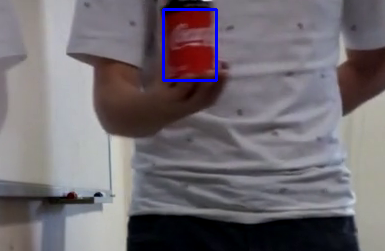
\includegraphics[width=0.7\textwidth]{../example_frame.png}
%	  \caption{voorbeeld van onze blikdetectie}
%	 \end{beamercolorbox}
%
%	\end{figure}
%		\justifying
%		Nunc mi felis, mattis eu nunc sit amet, convallis posuere felis. Pellentesque a ligula arcu. Ut viverra ipsum et sodales malesuada. Pellentesque lobortis luctus quam non tincidunt. Praesent in cursus purus. 
%		
%			\begin{block}{Block}
%			\begin{center}
%			Formula 1: \hspace{2em}	$\alpha=\gamma, \sum_{i}$
%			
%			Formula 2:	\hspace{2em} $\beta=\gamma^2+\epsilon$
%			\end{center}
%			\end{block}
%	
%		\vspace{0.5em}
%		{\bfseries Title 2}
%		
%		Integer erat nibh, fermentum ac sem nec, luctus imperdiet risus. Suspendisse eget velit massa. Pellentesque varius eu nisi sed auctor. Vestibulum ante ipsum primis in faucibus orci luctus et ultrices posuere cubilia Curae; Pellentesque a blandit tortor. In at eleifend ante, id bibendum mi. 
%		
%		\begin{proof}{Proof.}
%		Content
%		\end{proof}
%		
%		Praesent sit amet molestie enim. Sed laoreet hendrerit leo, in eleifend elit molestie sed. Donec hendrerit tristique enim, vel porttitor dui fringilla aliquet. Nullam at turpis ac dui viverra lacinia. Vivamus rutrum, diam non vehicula sodales, quam enim cursus dolor, id egestas velit elit nec neque. 
%		
%		\begin{alertblock}{Alert block}
%		See beamer template for additional blocks
%		\end{alertblock}
%		
%		\begin{enumerate}
%		\item some item
%		\item other item
%		\item more items 
%			\begin{enumerate}
%			\item some item
%			\item other item
%				\begin{enumerate}
%				\item more items 
%				\end{enumerate}
%			\item ...
%			\end{enumerate}
%		\item ...
%		\end{enumerate}
%	
%		 Nulla mattis interdum nibh, eu euismod mauris facilisis sed. Phasellus aliquam mattis sem, in dignissim enim vehicula in. Etiam condimentum efficitur massa at vulputate.
%	\end{column}
\end{columns}

\end{frame}
\end{document}
